% =====================================================================
\section{Шина I\texorpdfstring{\textsuperscript{2}}{2}C: экран}
\label{les:i2c}
% =====================================================================
\lessonintro
  {разобраться, как по двум проводам общаются несколько устройств, и вывести информацию на OLED-экран}
  {урок~\ref{les:signals} (цифровой сигнал), урок~\ref{les:gpio-in} (подтяжка), урок~\ref{les:adc} (потенциометр)}
  {вольтметр с экраном: напряжение крупными цифрами и полоска-шкала}
  {OLED-дисплей SSD1306 128×64 с интерфейсом I\textsuperscript{2}C, потенциометр \SI{10}{k\ohm}}

\subsection{Два провода на всех}

Экрану нужно передать много данных --- целую картинку. Можно было бы использовать UART, но у него
есть недостаток: он соединяет только \emph{два} устройства. А если к плате нужно подключить экран,
датчик температуры и часы? Для этого придумали шину \textbf{I\textsuperscript{2}C} (читается «ай-ту-си»,
от англ. \emph{Inter-Integrated Circuit}).

Всего два провода:
\begin{itemize}
  \item \textbf{SDA} (\emph{Serial Data}) --- по нему идут данные;
  \item \textbf{SCL} (\emph{Serial Clock}) --- «метроном»: ведущее устройство отбивает такт, и все знают,
        когда читать очередной бит. Поэтому, в отличие от UART, договариваться о скорости заранее не нужно.
\end{itemize}

На шине одно \textbf{ведущее} устройство (наша плата) и несколько \textbf{ведомых}. У каждого ведомого
свой \textbf{адрес} --- число от 8 до 119. Ведущий начинает разговор словами «эй, устройство номер 0x3C!»,
и отвечает только то, чей это адрес. Как учитель, который вызывает учеников по фамилии.

\begin{figure}[H]
\centering
\begin{circuitikz}[scale=0.95,transform shape]
  \draw (0,4.4) node[vcc]{3,3 В} -- (0,4.2) -- (3,4.2);
  \draw (1.5,4.2) to[R,l_=\SI{4.7}{k\ohm}] (1.5,2.8) coordinate(sdaR);
  \draw (3,4.2) to[R,l=\SI{4.7}{k\ohm}] (3,1.8) coordinate(sclR);
  \draw[thick,accent] (-1,2.8) node[left,text=accent]{SDA} -- (13,2.8);
  \draw[thick,esp] (-1,1.8) node[left,text=esp]{SCL} -- (13,1.8);
  \fill (sdaR) circle (1.5pt); \fill (sclR) circle (1.5pt);
  \node[blk,fill=blkcpu,minimum width=2.2cm,minimum height=1.2cm] (m) at (0,0) {ESP32-S3\\ \scriptsize ведущий};
  \node[blk,fill=blkper,minimum width=2.2cm,minimum height=1.2cm] (d1) at (5,0) {Экран\\ \scriptsize адрес 0x3C};
  \node[blk,fill=blkper,minimum width=2.2cm,minimum height=1.2cm] (d2) at (8.2,0) {Термометр\\ \scriptsize адрес 0x76};
  \node[blk,fill=blkper,minimum width=2.2cm,minimum height=1.2cm] (d3) at (11.4,0) {…\\ \scriptsize до 112 адресов};
  \foreach \d in {m,d1,d2,d3}{
    \draw[accent] ($(\d.north)+(-0.3,0)$) -- ($(\d.north)+(-0.3,0)$ |- 0,2.8) node[circle,fill,inner sep=1.2pt]{};
    \draw[esp] ($(\d.north)+(0.3,0)$) -- ($(\d.north)+(0.3,0)$ |- 0,1.8) node[circle,fill,inner sep=1.2pt]{};
  }
  \node[font=\sffamily\scriptsize] at (0,-1) {SDA = \pin{8}, SCL = \pin{9}};
\end{circuitikz}
\caption{Шина I\textsuperscript{2}C: одна пара проводов, много устройств}
\end{figure}

Устройства на шине не выдают 1 --- они умеют только притягивать линию к земле (0). А единицу создают
\textbf{подтягивающие резисторы} --- точно так же, как у кнопки из урока~\ref{les:gpio-in}. Благодаря этому,
даже если два устройства заговорят одновременно, ничего не сгорит. На модулях экранов и датчиков
подтягивающие резисторы обычно уже распаяны.

\subsection{Как выглядит разговор по I\texorpdfstring{\textsuperscript{2}}{2}C}

\begin{figure}[H]
\centering
\begin{tikzpicture}[x=0.72cm,y=0.8cm]
  \node[left,text=esp,font=\sffamily\small] at (0,3) {SCL};
  \draw[very thick,esp] (0,3.8) -- (2,3.8) -- (2.5,3.8) -- (2.5,2.6)
    \foreach \k in {0,...,8}{ -- ({3+\k*2},2.6) -- ({3+\k*2},3.8) -- ({4+\k*2},3.8) -- ({4+\k*2},2.6) }
    -- (21.5,2.6) -- (21.5,3.8) -- (23.5,3.8);
  \node[left,text=accent,font=\sffamily\small] at (0,1) {SDA};
  \draw[very thick,accent] (0,1.6) -- (1.2,1.6) -- (1.2,0.4) -- (2.8,0.4);
  \foreach \k/\l in {0/A6,1/A5,2/A4,3/A3,4/A2,5/A1,6/A0,7/R/W,8/ACK}{
    \pgfmathsetmacro{\xa}{2.8+\k*2}
    \draw[thick,accent] (\xa,0.4) -- (\xa+0.2,1.6) -- (\xa+1.8,1.6) -- (\xa+2,0.4);
    \draw[thick,accent] (\xa,1.6) -- (\xa+0.2,0.4) -- (\xa+1.8,0.4) -- (\xa+2,1.6);
    \node[font=\sffamily\scriptsize] at (\xa+1,1) {\l};
  }
  \draw[very thick,accent] (20.8,0.4) -- (22.3,0.4) -- (22.3,1.6) -- (23.5,1.6);
  \draw[dashed,gray] (1.2,0) -- (1.2,4.3) node[above,font=\sffamily\scriptsize,text=black]{СТАРТ};
  \draw[dashed,gray] (22.3,0) -- (22.3,4.3) node[above,font=\sffamily\scriptsize,text=black]{СТОП};
  \draw[decorate,decoration={brace,mirror,amplitude=4pt}] (2.8,-0.1) -- (16.8,-0.1) node[midway,below=5pt,font=\sffamily\scriptsize]{7-битный адрес: «кого зову»};
  \draw[decorate,decoration={brace,mirror,amplitude=4pt}] (16.8,-0.1) -- (18.8,-0.1) node[midway,below=5pt,font=\sffamily\scriptsize,align=center]{читать\\ или писать};
  \draw[decorate,decoration={brace,mirror,amplitude=4pt}] (18.8,-0.1) -- (20.8,-0.1) node[midway,below=5pt,font=\sffamily\scriptsize,align=center]{«я тут!»\\ (ACK)};
\end{tikzpicture}
\caption{Начало разговора по I\textsuperscript{2}C. Данные на SDA меняются, пока SCL = 0, и читаются,
пока SCL = 1. Ведомое устройство подтверждает, что услышало, --- притягивает SDA к 0 (ACK)}
\end{figure}

\subsection{Подключаем экран}

OLED-экран состоит из $128 \times 64 = 8192$ крошечных светящихся точек --- \textbf{пикселей}. Подключим
его к плате: SDA → \pin{8}, SCL → \pin{9}, питание --- от 3,3~В. Экран удобно разместить над макетной
платой и соединить проводами «мама--папа».

\begin{twoview}{Подключение OLED-экрана к шине I\textsuperscript{2}C}{fig:oled}
\begin{tikzpicture}[bb]
  \bbBoard{24}
  \bbDevKit{29}{25}
  \bbOLED{3}{21}
  \draw[wire=wblack] (3,21) -- (3,16);
  \draw[wire=wred] (4,21) -- (4,17);
  \draw[wire=wyellow] (5,21) -- (5,19.5) -- (27.8,19.5) -- (27.8,11) -- (dk-9);
  \draw[wire=wblue] (6,21) -- (6,20.2) -- (28.4,20.2) -- (28.4,14) -- (dk-8);
  \draw[wire=wblack] (dk-GND) -- (26.5,4) -- (26.5,16) -- (24,16);
  \draw[wire=wred] (dk-3V3) -- (28.8,25) -- (28.8,33) -- (-2,33) -- (-2,17) -- (1,17);
\end{tikzpicture}
\nextview
\begin{circuitikz}
  \node[draw,thick,fill=blkcpu,minimum width=2.6cm,minimum height=3.2cm,label={[font=\sffamily\bfseries]above:ESP32-S3}] (a) at (0,0) {};
  \node[draw,thick,fill=blkper,minimum width=2.6cm,minimum height=3.2cm,label={[font=\sffamily\bfseries]above:OLED SSD1306}] (b) at (7,0) {};
  \draw ($(a.east)+(0,1.1)$) node[left,font=\scriptsize]{3V3} -- ($(b.west)+(0,1.1)$) node[right,font=\scriptsize]{VCC};
  \draw[accent] ($(a.east)+(0,0.4)$) node[left,font=\scriptsize,text=black]{\pin{8}} -- node[above,font=\scriptsize]{SDA} ($(b.west)+(0,0.4)$) node[right,font=\scriptsize,text=black]{SDA};
  \draw[esp] ($(a.east)+(0,-0.3)$) node[left,font=\scriptsize,text=black]{\pin{9}} -- node[above,font=\scriptsize]{SCL} ($(b.west)+(0,-0.3)$) node[right,font=\scriptsize,text=black]{SCL};
  \draw ($(a.east)+(0,-1.1)$) node[left,font=\scriptsize]{GND} -- ($(b.west)+(0,-1.1)$) node[right,font=\scriptsize]{GND};
\end{circuitikz}
\end{twoview}

\begin{caution}
Порядок выводов у разных экранов бывает разным: GND--VCC--SCL--SDA или VCC--GND--SCL--SDA.
Перед подключением прочитай подписи на своём модуле!
\end{caution}

\subsection{Сканер шины}

Первое, что стоит сделать с новым модулем, --- проверить, отвечает ли он, и узнать его адрес.
Программа-сканер по очереди «вызывает» все адреса и сообщает, кто откликнулся:

\codecap{Сканер I\textsuperscript{2}C}
\codeinput{l12_scanner}

Для экрана SSD1306 обычно увидишь адрес \code{0x3C}. Если не нашлось ничего --- проверь провода и
не перепутаны ли SDA и SCL.

\subsection{Первая надпись на экране}

Установи через \textsf{Tools → Manage Libraries} библиотеки \textbf{Adafruit SSD1306} и \textbf{Adafruit GFX}.
Библиотека рисует картинку в памяти платы, а команда \code{display()} отправляет её на экран целиком.

\begin{figure}[H]
\centering
\begin{tikzpicture}[x=0.9mm,y=-0.9mm]
  \fill[black] (-2,-2) rectangle (130,66);
  \foreach \x in {0,8,...,128} \draw[gray!40,very thin] (\x,0) -- (\x,64);
  \foreach \y in {0,8,...,64} \draw[gray!40,very thin] (0,\y) -- (128,\y);
  \node[anchor=north west,font=\ttfamily\bfseries\Large,text=cyan!40,inner sep=0] at (2,2) {ESP32-S3};
  \node[anchor=north west,font=\ttfamily\small,text=cyan!40,inner sep=0] at (2,32) {uptime: 42 s};
  \fill[esp] (0,0) circle (1.3);
  \node[font=\sffamily\scriptsize,anchor=south,text=black] at (0,-3) {(0, 0)};
  \node[font=\sffamily\scriptsize,anchor=south,text=black] at (128,-3) {(127, 0)};
  \node[font=\sffamily\scriptsize,anchor=north,text=black] at (0,67) {(0, 63)};
  \draw[->,thick,esp] (0,-8) -- node[above,font=\sffamily\scriptsize,text=black]{$x$ растёт вправо} (40,-8);
  \draw[->,thick,esp] (-8,0) -- node[left,font=\sffamily\scriptsize,text=black,align=right]{$y$ растёт\\ вниз} (-8,30);
\end{tikzpicture}
\caption{Координаты пикселей экрана: начало --- в левом верхнем углу, и $y$ растёт \emph{вниз}}
\end{figure}

\codecap{Надпись на OLED-экране}
\codeinput{l12_oled_hello}

\begin{tip}
Стандартные шрифты Adafruit GFX не содержат русских букв --- для кириллицы нужны специальные шрифты
или библиотека U8g2. В примерах обойдёмся латиницей.
\end{tip}

\subsection{Практика: вольтметр с экраном}

Соединим экран с потенциометром из урока~\ref{les:adc}: на экране будет напряжение на движке крупными
цифрами и полоска-шкала, как у настоящего прибора.

\begin{figure}[H]
\centering
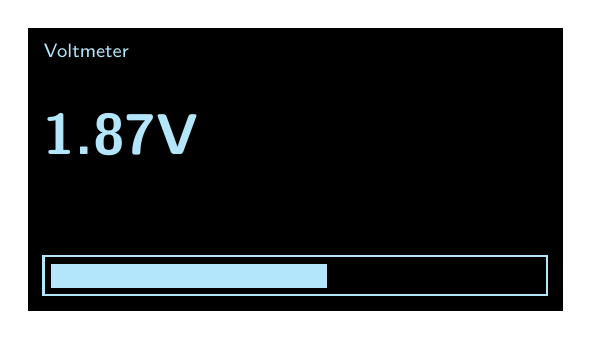
\begin{tikzpicture}[x=0.5mm,y=-0.5mm]
  \fill[black] (-4,-4) rectangle (132,68);
  \node[anchor=north west,font=\sffamily\scriptsize,text=cyan!30,inner sep=0] at (0,0) {Voltmeter};
  \node[anchor=north west,font=\sffamily\bfseries\huge,text=cyan!30,inner sep=0] at (0,18) {1.87V};
  \draw[cyan!30,thick] (0,54) rectangle (128,64);
  \fill[cyan!30] (2,56) rectangle (72,62);
\end{tikzpicture}
\caption{Экран вольтметра: заголовок, напряжение крупно и полоска}
\end{figure}

\begin{twoview}{Вольтметр: потенциометр на GPIO1 и экран на I\textsuperscript{2}C}{fig:voltmeter}
\begin{tikzpicture}[bb]
  \bbBoard{24}
  \bbDevKit{29}{25}
  \bbOLED{3}{21}
  \bbPotD{12}{12}{10k}
  \draw[wire=wblack] (12,14) -- (12,16);
  \draw[wire=wred] (14,14) -- (14,17);
  \draw[wire=wgreen] (dk-1) -- (39.5,22) -- (39.5,32.2) -- (13,32.2) -- (13,14);
  \draw[wire=wblack] (3,21) -- (3,16);
  \draw[wire=wred] (4,21) -- (4,17);
  \draw[wire=wyellow] (5,21) -- (5,19.5) -- (27.8,19.5) -- (27.8,11) -- (dk-9);
  \draw[wire=wblue] (6,21) -- (6,20.2) -- (28.4,20.2) -- (28.4,14) -- (dk-8);
  \draw[wire=wblack] (dk-GND) -- (26.5,4) -- (26.5,16) -- (24,16);
  \draw[wire=wred] (dk-3V3) -- (28.8,25) -- (28.8,33) -- (-2,33) -- (-2,17) -- (1,17);
\end{tikzpicture}
\nextview
\begin{circuitikz}
  \node[draw,thick,fill=blkcpu,minimum width=2.6cm,minimum height=3.6cm,label={[font=\sffamily\bfseries]above:ESP32-S3}] (a) at (0,0) {};
  \node[draw,thick,fill=blkper,minimum width=2.4cm,minimum height=1.6cm,font=\sffamily] (b) at (7,1) {OLED};
  \draw[accent] (1.3,1.3) node[left,font=\scriptsize,text=black]{\pin{8}} -- node[above,font=\scriptsize]{SDA} (5.8,1.3);
  \draw[esp] (1.3,0.7) node[left,font=\scriptsize,text=black]{\pin{9}} -- node[below,font=\scriptsize]{SCL} (5.8,0.7);
  \draw (7,1.8) -- (7,2.2) node[vcc]{3,3 В};
  \draw (7,0.2) -- (7,-0.1) node[ground]{};
  \draw (5,-4.4) node[ground]{} to[pR,n=pot,l=\SI{10}{k\ohm}] (5,-1.7) -- (5,-1.5) node[vcc]{3,3 В};
  \draw (1.3,-1.4) node[left,font=\scriptsize]{\pin{1}} -- (3.8,-1.4) |- (pot.wiper);
\end{circuitikz}
\end{twoview}

\codecap{Вольтметр с экраном}
\codeinput{l12_voltmeter_oled}

Экран обновляется 10 раз в секунду --- чаще не нужно: глаз всё равно не заметит разницы
(вспомни инерцию зрения из урока~\ref{les:pwm}), а отправка картинки по шине занимает время.

\begin{summary}
\begin{itemize}[leftmargin=*]
  \item I\textsuperscript{2}C --- два провода (SDA и SCL), подтягивающие резисторы и адреса устройств.
  \item С новым модулем сначала запускаем сканер и узнаём адрес.
  \item Библиотека экрана рисует в памяти, \code{display()} отправляет картинку целиком.
  \item Координаты пикселей начинаются в левом верхнем углу, $y$ растёт вниз.
\end{itemize}
\end{summary}

\begin{quiz}
\begin{enumerate}
  \item Сколько проводов нужно, чтобы подключить к плате три устройства I\textsuperscript{2}C (не считая питания)?
  \item Как ведущее устройство выбирает, с кем разговаривать?
  \item В каком углу экрана пиксель с координатами (127, 63)?
\end{enumerate}
\end{quiz}

\begin{tasks}
\begin{enumerate}
  \item Нарисуй на экране смайлик с помощью \code{drawCircle()} и \code{fillCircle()}.
  \item Сделай «осциллограф»: рисуй график напряжения на ручке за последние 128 измерений.
  \item Покажи на экране IP-адрес платы из урока~\ref{les:radio} и «записку», пришедшую через веб-страницу (урок~\ref{les:web}).
\end{enumerate}
\end{tasks}
